\documentclass[11pt]{article}

\usepackage{hyperref}
\usepackage{xcolor}
\usepackage{graphicx}
\usepackage{tikz}
\usepackage{fontspec}
\usepackage{fontawesome5}
\usepackage{titlesec}
\usepackage{enumitem}
\usepackage{fancybox}
\hypersetup{hidelinks}

%%%%%%%%%%%%%%%%%%%%
% 设置
%%%%%%%%%%%%%%%%%%%%

\setlength{\parindent}{0pt}                 % 取消全局段落缩进
\pagenumbering{gobble}                      % 取消页码显示
\setlist[itemize]{nosep                     % 取消 itemize 的默认间距
	, before={\vspace*{-\parskip}}          % 取消 itemize 和后续段落之间的空白
	, leftmargin=*}                         % 取消 itemize 的左边距
\setlist[enumerate]{
	leftmargin=*,                           % 取消 enumerate 的左边距
	before={\vspace*{-\parskip}}}           % 取消 enumerate 和后续段落之间的空白
\renewcommand{\arraystretch}{1.2}           % 设置表格行间距
\linespread{1.25}                           % 设置正文行间距

\titleformat{\section}                      % 将原标题前面的数字取消了
{\LARGE\bfseries\raggedright}               % 字体改为 LARGE，bold，左对齐
{}{0em}                                     % 可用于添加全局标题前缀
{}                                          % 可用于添加代码
[{\color{secondary_color}\titlerule}]       % 标题下方加一条线
\titlespacing*{\section}{0cm}{*1.2}{*1.2}  % 标题左边留白，上方，下方

\usepackage[
a4paper,
left=1.2cm,
right=1.2cm,
top=1.5cm,
bottom=1cm,
nohead
]{geometry}                                 % 页面边距设置

% 字体设置
\setmainfont[
Path=fonts/,
Extension=.otf,
BoldFont=*-Bold,
]{NotoSerifSC}

% 自定义颜色
\definecolor{primary_color}{RGB}{200, 60, 60}    % 主色调（红）
\definecolor{secondary_color}{RGB}{200, 68, 28}  % 辅色调（橙红）

\newlength{\iconwidth}
\setlength{\iconwidth}{1.5em}               % 设置 section 标题部分图标占用的宽度

%%%%%%%%%%%%%%%%%%%%
% 文章内容
%%%%%%%%%%%%%%%%%%%%

% 学院
\newcommand{\school}{数学与计算科学学院}

% 联系方式
\newcommand{\contact}{
	\footnotesize
	\textcolor{white}{
		\faEnvelope \quad \href{mailto:lianghe@smail.xtu.edu.cn}{lianghe@smail.xtu.edu.cn}
		\hspace{4em}
		\faPhone \quad 17773031823
	}
}

\begin{document}
	
	%%%%%%%%%%%%%%%%%%%%
	% 页眉、页脚和背景
	%%%%%%%%%%%%%%%%%%%%
	
	% 页眉：校标组合+学院名
	\begin{tikzpicture}[remember picture, overlay]
		\node[anchor=north, inner sep=0pt](header) at (current page.north){
			
\includegraphics[width=\paperwidth]{images/head.png}
		};
		\node[anchor=west](school_logo) at (header.west){
			\hspace{0.5cm}
			
\includegraphics[width=0.2\textwidth]{images/nbu_logo.png}
		};
		\node[anchor=east](school_name) at(header.east){
			\textcolor{white}{\textbf{\school}}
			\hspace{0.5cm}
		};
	\end{tikzpicture}
	\vspace{-3.5em}
	
	% 页脚：联系方式
	\begin{tikzpicture}[remember picture, overlay]
		\node[anchor=south, inner sep=0pt](footer) at (current page.south){
			
\includegraphics[width=\paperwidth]{images/foot.png}
		};
		\node[anchor=center] at(footer.center){\contact};
	\end{tikzpicture}
	
	% 背景
	\begin{tikzpicture}[remember picture, overlay]
		\node[opacity=0.05] at(current page.center){
			
\includegraphics[width=0.7\paperwidth, keepaspectratio]{images/nbu_logo2.png}
		};
	\end{tikzpicture}
	
	%%%%%%%%%%%%%%%%%%%%
	% 简历正文
	%%%%%%%%%%%%%%%%%%%%
	
	% 左侧：个人信息 + 教育背景，占 78%
	\begin{minipage}[t]{0.78\textwidth}
		
		% 个人信息
		\section[个人信息]{\makebox[\iconwidth][c]{\color{primary_color}{\faAddressCard}}\quad 个人信息}
		
		\begin{tabular}{@{} p{0.50\linewidth} p{0.44\linewidth} @{}}
			\textbf{姓\qquad 名}：何亮      & \textbf{性\qquad 别}：男          \\[0.4em]
			\textbf{出生年月}：1998年5月8日  & \textbf{电\qquad 话}：17773031823 \\[0.4em]
			\multicolumn{2}{@{}l}{\textbf{邮\qquad 箱}：lianghe@smail.xtu.edu.cn} \\[0.4em]
		\end{tabular}
		
		\vspace{0.2em}
		\textbf{个人综述}：计算数学博士，专注偏微分方程的高效数值方法及其在计算固体力学与 \\
		拓扑优化中的应用，具备从理论推导到软件实现的全流程能力。参与多项校企合作 \\
		项目，擅长面向对象的高性能数值计算框架与程序开发，致力于将前沿计算数学理\\
		论转化为可扩展的高性能科学计算平台。
		\vspace{1em}
		
		% 教育背景
		\section[教育背景]{\makebox[\iconwidth][c]{\color{primary_color}{\faGraduationCap}}\quad 教育背景}
		
		\vspace{0.5em}
		
		{\large \textbf{湖南工程学院}}，大学本科，信息与计算科学专业 \hfill 2016年9月--2020年6月
		
		\vspace{0.5em}
		{\large \textbf{上海师范大学}}，硕士研究生，运筹学与控制论专业 \hfill 2020年9月--2023年6月
		
		\vspace{0.5em}
		{\large \textbf{湘潭大学}}，博士研究生，数学专业 \hfill 2023年9月--2026年6月\par
		\begin{itemize}
			\item \textbf{研究方向}：微分方程数值方法及应用（拓扑优化高效数值算法分析与实现）
			\item \textbf{导\qquad 师}：魏华祎 教授
		\end{itemize}
		
		\vspace{1.2em}
		
	\end{minipage}
	\hfill
	% 右侧：照片，占 20%
	\begin{minipage}[t]{0.2\textwidth}
		\vspace{2.5em}
		\setlength{\fboxsep}{0pt}
		\doublebox{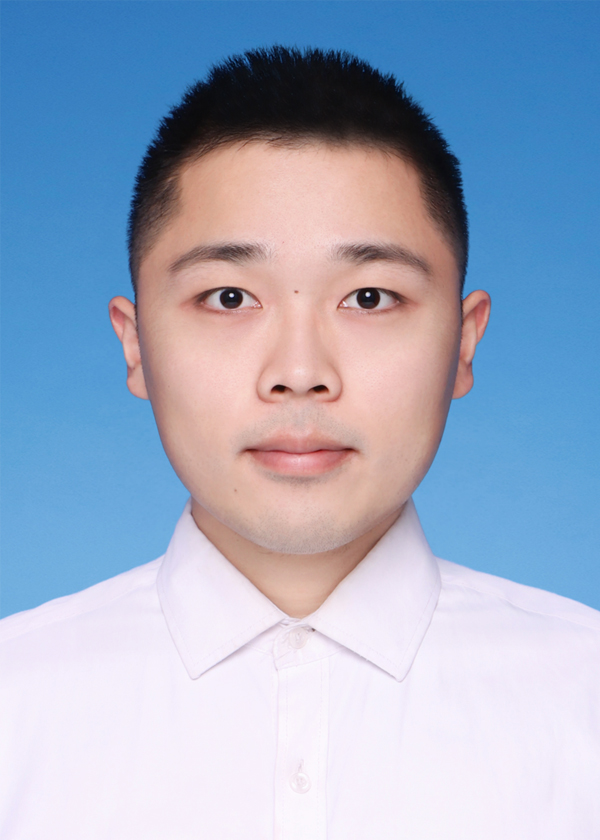
\includegraphics[width=\linewidth]{images/heliang.jpg}}
	\end{minipage}
	
	% 学术论文
	\begin{minipage}[t]{\textwidth}
		\section[学术论文]{\makebox[\iconwidth][c]{\color{primary_color}{\faFile}}\quad 学术论文}
		
		\vspace{0.5em}
		
		\begin{enumerate}[label={[\arabic*]}, leftmargin=2.5em]
			\setlength{\itemsep}{0.2em}
			
			\item \textbf{Liang He}, Huayi Wei, Tian Tian. SOPTX: A Modular and Extensible Framework for Topology Optimization with Multi-Backend Support[J]. \textit{Communications in Computational Physics}，已录用。
			
			\item Tian Tian, Chunyu Chen, \textbf{Liang He}, Huayi Wei. Adaptive finite element method for phase field fracture models based on recovery error estimates[J]. \textit{Journal of Computational and Applied Mathematics}, 472 (2026): 116732.
			
			\item Yangyang Zheng, Huayi Wei, Yunqing Huang, Chunyu Chen, Tian Tian, Hanbin Liu, Wenbin Wang, \textbf{Liang He}. FEALPy: A Cross-platform Intelligent Numerical Simulation Engine[J]. \textit{Communications in Computational Physics}，已录用。
		\end{enumerate}
		
		\vspace{0.6em}
	\end{minipage}
	
	% 软件著作权
	\begin{minipage}[t]{\textwidth}
		\section[软件著作权]{\makebox[\iconwidth][c]{\color{primary_color}{\faCopyright}}\quad 软件著作权}
		
		\vspace{0.5em}
		
		\begin{enumerate}[label={[\arabic*]}, leftmargin=2.5em]
			\setlength{\itemsep}{0.2em}
			
			\item \textbf{结构拓扑优化仿真计算软件}\\[0.3em]
			\textbf{专利申请号}：2025SR0887352 \qquad \textbf{专利授权号}：软著登字第 15543550 号 \qquad \textbf{贡献}：第一完成人
			
			\item \textbf{建筑结构力学仿真计算软件}\\[0.3em]
			\textbf{专利申请号}：2024SR0961048 \qquad \textbf{专利授权号}：软著登字第 13364921 号 \qquad \textbf{贡献}：第三完成人
		\end{enumerate}
		
		\vspace{0.6em}
	\end{minipage}

	% 项目经历
	\begin{minipage}[t]{\textwidth}
		\section[项目经历]{\makebox[\iconwidth][c]{\color{primary_color}{\faChalkboardTeacher}}\quad 项目经历}
		
		\vspace{0.5em}
		
		{\large \textbf{建筑结构力学分析计算内核开发 (C++)}}\quad \textbf{主要参与人}
		\begin{itemize}
			\setlength{\itemsep}{0.2em}
			\item \textbf{项目简介}：本项目为与中国建筑第五工程局有限公司的合作课题，旨在研发一套跨平台、高可扩展\\
			且易于维护的底层建筑结构力学仿真计算内核。
			\item \textbf{核心职责}：负责 C++ 仿真计算内核的底层代码设计与实现；深度参与并承担计算结果严格物理对标\\
			与验证的核心工作，并完成技术文档的最终交付。
		\end{itemize}
		
		\vspace{0.6em}
		
		{\large \textbf{CAX 仿真计算引擎 FEALPy 核心模块开发}}\quad \textbf{主要参与人}
		\begin{itemize}
			\setlength{\itemsep}{0.2em}
			\item \textbf{项目简介}：参与维护并开发开源数值仿真引擎 FEALPy (\href{https://github.com/weihuayi/fealpy}{https://github.com/weihuayi/fealpy})，\\
			该平台致力于为偏微分方程提供高效、灵活的科学计算支持。
			\item \textbf{核心职责}：主导设计并实现了计算固体力学核心算法模块；完成了包含线弹性方程、弹塑性方程\\
			在内的多种力学求解器的底层封装，大幅提升了引擎在固体力学领域的计算能力。
		\end{itemize}
		
		\vspace{0.6em}
		
		{\large \textbf{韶峰天工 CAX 智能工作流协作平台开发}}\quad \textbf{核心研发骨干}
		\begin{itemize}
			\setlength{\itemsep}{0.2em}
			\item \textbf{项目简介}：本项目旨在打造支撑 CAX 产学研用一体化的国产智能工作流协作平台，深度适配国产\\
			操作系统与异构算力，为智能制造与数字孪生提供坚实的工业软件底座。
			\item \textbf{核心职责}：负责平台结构工程领域核心计算节点的底层开发与封装；完成了桁架塔静力分析模块的\\
			开发与数值验证工作；参与针对弯管及三通管二次流抑制与压损优化的形状优化算法研发。
		\end{itemize}
		
		\vspace{1.2em}
	\end{minipage}
	
\end{document}